% !TeX root = ../praktikum.tex
% !TeX encoding = UTF-8
% !Tex spellcheck = de_DE



\subsection{Untersuchungen an Gittern}
In diesem Abschnitt werden verschiedene Gitter des Objektes 3 untersucht. Dazu wurde das entsprechende Dia in der Objektebene montiert. Das gewünschte Motiv auf der Schablone wurde möglichst mittig in dem Strahl montiert. Mit einer Papierschablone wurde verhindert, das Motive beleuchtet werden, die gerade nicht untersucht wurden, da dies eine Überlagerung mehrerer Fourierspektren zur Folge hätte (vgl. Abb.~\ref{fig:kreuzgitter_und_spektrum}~b und c) und das Untersuchen eines einzelnen Spektrums unmöglich machen würde. Für jedes der neun Motive wurde je ein Bild in der Fourierebene sowie in der Abbildungsebene aufgenommen. Beim Einschieben der Objekte ließ sich feststellen, dass die Bewegungsrichtung der Abbildung entgegengesetzt zu der des echten Motivs ist. Ebenso sieht man bei asymmetrischen Objekten, dass diese "auf dem Kopf stehen".


\begin{figure}[ht]
	\centering
	%\includegraphicsRS[width=0.6\textwidth]{images/Regina/abb13.jpg}
	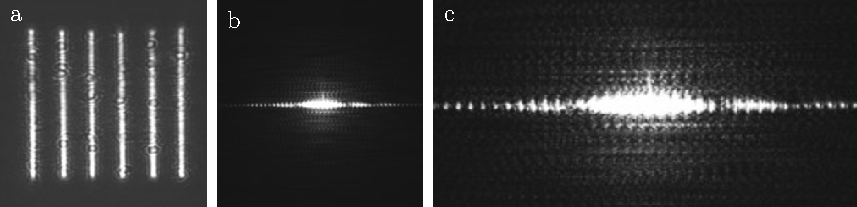
\includegraphics{images/Regina/abb13.pdf}
	\caption[Gitter mit Fourierspektrum]{
		Vertikales Gitter (a) und das dazugehörige Beugungsbild (b), welches das Fourierspektrum darstellt. Das Fourierspektrum weist erneut Beugungsbilder als eine Unterstruktur auf (c).
	}
	\label{fig:gitter_und_spektrum}
\end{figure}

Für eines der Gittermotive aus der ersten Reihe sind diese Aufnahmen in Abbildung~\ref{fig:gitter_und_spektrum} abgebildet. In der Fourierebene ist eine Reihe von Punkten zu sehen. Die Motive der zweiten Reihe ergeben in beiden Ebenen jeweils das gleiche Bild, jedoch um $90^\circ$ gedreht. Je dichter die Gitterlinien beieinander liegen, desto weiter liegen die Punkte in der Fourierebene auseinander.

Die Abbildung eines Motivs der letzten Reihe (Kreuzgitter) ist in Abbildung~\ref{fig:kreuzgitter_und_spektrum}~a abgebildet, b zeigt das Bild in der Fourierebene (\textit{Fourierspektrum}). Zusätzlich zeigt die Abbildung~\ref{fig:kreuzgitter_und_spektrum}c das Fourierspektrum, wenn mehrere Motive gleichzeitig beleuchtet werden. Die Kreuzgitter erzeugen in der Fourierebene zwei senkrechte Punktreihen, wobei der Punktabstand mit zunehmenden Gitterlinienabstand abnimmt.

\begin{figure}[ht]
	\centering
	%\includegraphicsRS[width=0.4\textwidth]{images/Regina/abb14.jpg}
	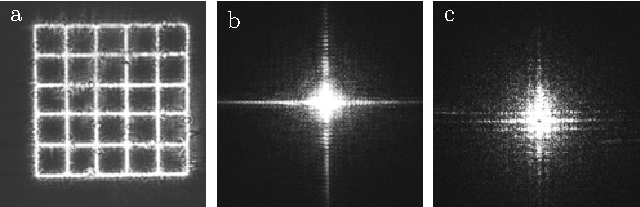
\includegraphics{images/Regina/abb14.pdf}
	\caption[Kreuzgitter mit Fourierspektrum]{
		Kreuzgitter (a) und das dazugehörige Beugungsbild (b), das das Fourierspektrum darstellt. Eine Überlagerung von mehreren Fourierspektren (c).
	}
	\label{fig:kreuzgitter_und_spektrum}
\end{figure}



\subsubsection*{Auswertung}
Das Zustandekommen und Aussehen einer Abbildung kann durch die aus der zweifachen 
%TODO: ich hab hier jetzt mal nich weitergemacht, da ich auf die Schnelle nich ganz verstanden hab, was du hier sagen willst ;)
Da das Licht im vertikalen Gitter nur in der vertikalen Richtung gebeugt wird, bilden sich die Intensitätsschwankungen in der Fourierebene ausschließlich in horizontaler Richtung aus. Somit wurde dort eine senkrecht zum Gitter stehende Reihe aus Interferenzmaxima und -minima beobachtet, vgl. Abbildung~\ref{fig:gitter_und_spektrum}. Das Drehen des Motivs sorgt ebenfalls für ein gedrehtes Bild in der Fourierebene. Dies ist direkt aus der Beugungstheorie an Gittern ersichtlich. Die Änderungen des Spektrums, welche unter Variation des Spaltabstandes zu beobachten waren, lassen sich mit der mathematischen Eigenschaft der Ähnlichkeit der FT erklären (s. Abschnitt~\ref{chap:math_basic}). Allerdings folgt auch dies direkt aus der Beugungstheorie an Gittern, beziehungsweise Mehrfachspalten.\\

Bei einem Kreuzgitter findet die Beugung in horizontaler und vertikaler Richtung statt, welches einer Kreuzform in der Fourierebene entspricht. Das Motiv entspricht also einer Überlagerung zweier um $90^\circ$ gedrehten Gitter. Nach der mathematischen Eigenschaft der Linearität der FT (s. Abschnitt~\ref{chap:math_basic}) folgt somit auch die Überlagerung der entsprechenden Spektren. Dies war sehr gut zu beobachten.

Wenn mehrere Motive beleuchtet wurden, ergab sich in der Fourierebene die in Abbildung~\ref{fig:kreuzgitter_und_spektrum}~c dargestellte kreuzförmige Anordnung. Diese zeigt nicht ein einzelnes Kreuz, sondern mehrere Kreuze in bestimmtem Abstand zueinander. Das Auftreten mehrerer Kreuze lässt sich analog mit der Linearitätseigenschaft der FT erklären.

%TODO: guck dir bei gelegenheit mal den hier folgenden abschnitt an - die hohe intensität im zentrum ist doch immer die nullte beugundsordnung,, oder hab ich da was falsch verstanden? sollten wir das kind dann nich einfach mal beim namen nennen? s.u. passiert hier nämlich nicht... 
Sowohl beim vertikalen Gitter als auch bei dem Kreuzgitter ist in der Fourierebene im Zentrum der Beugungsbilder eine maximale Intensität zu erkennen. Dieses Maximum entsteht durch das Kreuzen der mittleren horizontalen oder im Fall des Kreuzgitters der vertikalen und horizontalen Beugungsbilder. Dabei ist bei jedem weiteren Kreuzpunkt erneut eine erhöhte Intensität zu erkennen, die nach außen hin abnimmt. Diese lässt sich ebenfalls bei einem
Doppelspalt beobachten, wobei das Intensitätsmaximum nullter Ordnung am stärksten ist und die Maxima höherer Ordnungen immer schwächer werden ($\nicefrac{sin(x)}{x}$). Dabei nimmt die Intensität im Zentrum mit zunehmend kleiner werdender Gitterkonstante zu.
Weiterhin wiesen alle Intensitätsmaxima eine Unterstruktur auf. Diese Unterstrukturen entstehen durch die Interferenz der Haupt- und Nebenmaxima aller Spalte des Gitters. Somit entsteht im Gegensatz zum Doppelspalt das Beugungsbild eines Gitter aus Vielfachinterferenzen. Diese Eigenschaft entspricht der mathematisch geforderten Linearität, denn das Beugungsbild eines Gitters kann somit durch das Aufsummieren der einzelnen Beugungsbilder des Einzelspaltes erzeugt werden (siehe Abschnitt \ref{chap:math_basic}).


\subsection{Erzeugung von Beugungsbildern von Punkten}

In diesem Abschnitt werden verschiedene Punktpaare des Objektes 2 untersucht. Das entsprechende Dia wurden hierzu analog zum vorangegangenen Abschnitt in der Objektebene montiert und das gewünschte Motiv entsprechend ausgeleuchtet. Die Abbildungen \ref{fig:punktpaare_verschieden_und_spektren} und \ref{fig:punktpaare_gleich_und_spektren} zeigen die hierzu aufgenommenen Bilder der Abbildungs- sowie der zugehörigen Fourierebene. 

\begin{figure}[h]
	\centering
	%\includegraphicsRS[width=0.3\textwidth]{images/Regina/abb15.jpg}
	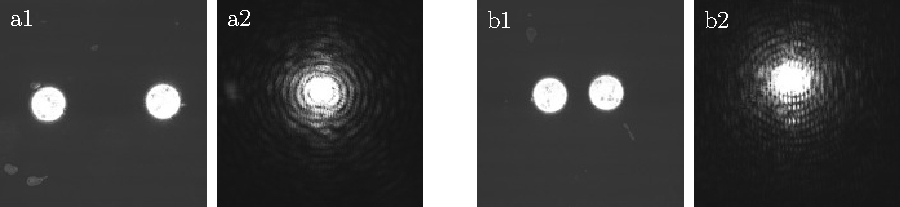
\includegraphics{images/Regina/abb15.pdf}
	\caption[Punktpaare unterschiedlicher Abstände und Fourierspektren]{
		Punktpaare mit unterschiedlichen Abständen zueinander (a1, b1) und die dazugehörigen Beugungsbilder in der Fourierebene (a2, b2).
	}
	\label{fig:punktpaare_verschieden_und_spektren}
\end{figure}

\begin{figure}[h]
	\centering
	%\includegraphicsRS[width=0.3\linewidth]{images/Regina/abb16.jpg}
	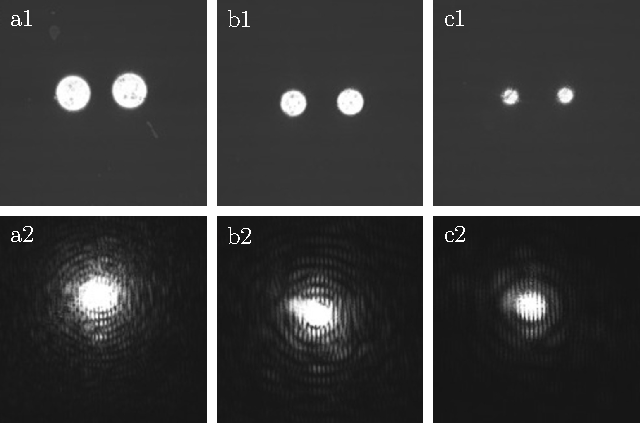
\includegraphics{images/Regina/abb16.pdf}
	\caption[Punktpaare gleicher Abstände und Fourierspektren]{
		Punktpaare mit gleichen Abständen und unterschiedlicher Größe (a1, b1, c1) und die dazugehörigen Beugungsbilder in der Fourierebene (a2, b2, c2).
	}
	\label{fig:punktpaare_gleich_und_spektren}
\end{figure}

Dabei scheinen sich die Beugungsbilder der Fourierebene aus zwei sich überlagernden jeweils von einem gemeinsamen Mittelpunkt ausgehenden Mengen von Kreisringen zusammenzusetzen. Die beiden Kreisringmittelpunkte liegen dabei in der gleichen Ebene wie das Punktpaar auf dem entsprechenden Dia. Durch die Überlagerung der beiden Kreisringgruppen entsteht im Beugungsbild ein oval wirkendes Interferenzbild. Wie sich dieses Oval mit zunehmendem Abstand der beiden Punkte auf dem Dia zueinander verändert, ist aufgrund der eher schlechten Auflösung der hierzu aufgenommenen Bilder nur schwer auszumachen (vgl. Abbildung \ref{fig:punktpaare_gleich_und_spektren}). 


\subsubsection*{Auswertung}

Bei der optischen Fouriertransformation gilt für Punkte, wie bereits für Gitter erläutert, die Linearität, sodass sich das erzeugte Beugungsbild in der Fourierebene aus der Summe der Beugungsbilder der einzelnen Punkte ergibt. Das Beugungsbild eines Punktes besteht aus konzentrischen Ringen, dessen Breite und Intensität nach außen abnehmen. Durch das Verschiebungtheorem der Fouriertransformation ist gegeben, dass sich das Beugungsbild der beiden Punkte an derselben Position befindet, trotz der unterschiedlichen Positionen der Punkte. Bei zwei Punkten ergibt sich somit eine Vielfachinterferenz analog zum Gitter, welches ebenfalls durch Unterstrukturen in den konzentrischen Ringen erkennbar wird (Abb.~\ref{fig:punktpaare_verschieden_und_spektren}~b, d). Mit zunehmendem Abstand zwischen den Punkten werden die Unterstrukturen feiner. Dies entspricht dem Ähnlichkeitstheorem (siehe Abschnitt \ref{eq:sim}), sodass sich die Beugungsmaxima mit zunehmendem Abstand der Punkte annähern, bzw. die Abstände zwischen den Maxima kleiner werden. Für ein Gitter bedeutet dieses, je größer die Gitterkonstante, d.h. je größer der Abstand zwischen den Spalten, desto kleiner wird der Abstand zwischen den einzelnen Maxima und Minima.

Beim geringsten Abstand sind im Beugungsbild neben den konzentrischen Formen auch vertikale Gitter zu erkennen (Abb.~\ref{fig:punktpaare_verschieden_und_spektren}~b2). Diese Gitterform stellen die bereits erwähnten Unterstrukturen der Beugungsbilder dar. Zwei Punkte ergeben in der Fourierebene als
Unterstruktur eine Linienstruktur senkrecht zur Verbindungslinie der beiden Punkte. Diese ergeben sich somit ebenfalls bei zwei Punkten mit höherem Abstand, sind aber wegen des kleinen Abstands zwischen den Spalten des vertikalen Gitters in der Fourierebene schlecht zu erkennen, da sich die Fouriertransformierte reziprok verhält (Ähnlichkeitstheorem). Bei kleinerem Abstand zwischen den Punkten vergrößert sich der Abstand der Spalte im vertikalen Gitter und wird dadurch erkennbar. Diese Unterstrukturen sind bei gleichbleibendem Abstand und kleinerer Größe der Punkte selbst noch ausgeprägter und damit besser zu erkennen (Abb.~\ref{fig:punktpaare_gleich_und_spektren}~b2, c2). Die Intensitätsmaxima sind bei den kleineren Punkten durch deren größeren Abstand zueinander kleiner ausgeprägt als bei den größeren Punkten. Somit weist das Hauptmotiv des Beugungsbilds eine geringe Intensität auf, wodurch die Unterstruktur einfacher zu erkennen
ist.
Auch im Beugungsbild eines Punktringes (Abb.~\ref{fig:punktringe_und_spektrum}) sind Unterstrukturen in der Fourierebene zu erkennen, welche sich durch die Anordnung der acht Punkte ergeben. Zwei Punkte weisen eine senkrechte Linienstruktur zur Verbindungslinie auf, sodass sich bei acht Punkten vier Linienstrukturen (horizontal, vertikal, beide Diagonale) ergeben. Wenn sich diese Strukturen kreuzen, ergeben sich acht Schnittpunkte und somit entstehen Unterstrukturen in Form von Achtecken (Abb.~\ref{fig:punktringe_ausschnitt}).

\begin{figure}[h]
	\centering
	%\includegraphicsRS[width=0.10\linewidth]{images/Regina/abb17.jpg}
	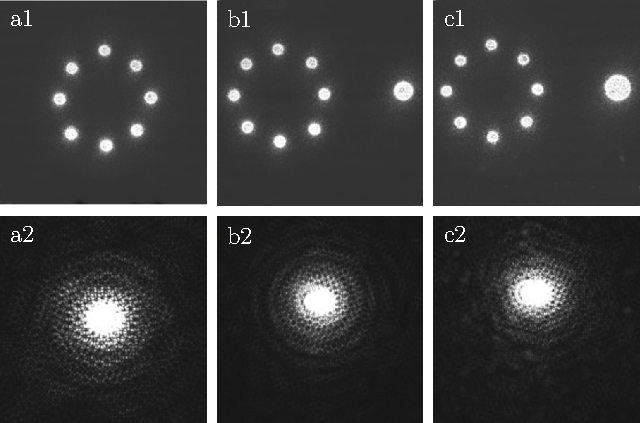
\includegraphics{images/Regina/abb17.pdf}
	\caption[Punktringe mit Fourierspektren]{
		Punktringe (a1) und Punktringe mit zusätzlichem Punkt in unterschiedlicher Größe (b1, c1) und die dazugehörigen Beugungsbilder in der Fourierebene (a2-c2).
	}
	\label{fig:punktringe_und_spektrum}
\end{figure}

\begin{figure}[h]
	\centering
	\includegraphicsRS[width=0.42\textwidth]{images/Regina/abb18.jpg}
	\caption[Beugungsbild der Punktringe mit Unterstruktur]{
		Ausschnitt aus dem Beugungsbild des Punktringes, welcher die Unterstruktur eines Achtecks zeigt.
	}
	\label{fig:punktringe_ausschnitt}
\end{figure}

Bei einem Punktkreis mit einem zusätzlichen Punkt ist das Beugungsbild nicht mehr symmetrisch und die Asymmetrie nimmt mit größer werdenden Punkten zu (Abb.~\ref{fig:punktpaare_gleich_und_spektren}~b, c).


\subsection{Erzeugung von Beugungsbilder von Buchstaben und Zahlen}

In diesem Abschnitt werden beispielhaft zwei der Motive des Objekts 4 und deren Beugungsbilder untersucht. Die Vorgehensweise zur Aufnahme der Abbildungen hierzu war analog zu den vorangegangenen Abschnitten. Abbildung \ref{fig:ziffern_mit_spektren} zeigt die gewählten Motive und deren Beugungsbilder. 

\begin{figure}[h]
	\centering
	%\includegraphicsRS[width=0.4\textwidth]{images/Regina/abb19.jpg}
	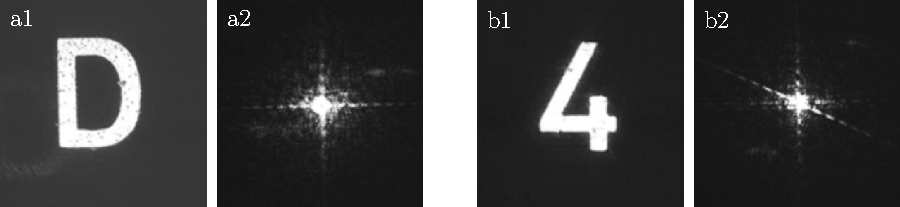
\includegraphics{images/Regina/abb19.pdf}
	\caption[Ziffern mit Fourierspektren]{
		Buchstabe D (a1) und Zahl 4 (b1) und die dazugehörigen Beugungsbilder in der Fourierebene (a2 und b2).
	}
	\label{fig:ziffern_mit_spektren}
\end{figure}

\subsubsection*{Auswertung}

Der Buchstabe D besteht sowohl aus horizontalen, sowie vertikalen Linien, als auch aus runden Elementen (Abb.~\ref{fig:ziffern_mit_spektren}~a1). Das Beugungsbild ergibt sich somit aus der Summe der Beugungsbilder dieser verschiedenen Formen. Die horizontalen Linien bilden ein Fourierspektrum in der Horizontalen und die vertikalen Linien in der Vertikalen mit den jeweiligen Maxima und Minima und Unterstrukturen (Abb.~\ref{fig:ziffern_mit_spektren}~a2). Die runde Form erzeugt im Beugungsbild konzentrische Ringe mit abnehmender Intensität, entsprechend dem Beugungsbild von Punkten. Da der Buchstabe D durch horizontale und vertikalen Linien dominiert wird, ist auch das Beugungsbild stark davon geprägt, sodass die konzentrischen Ringe durch eine geringere Intensität auch schlechter zu erkennen sind.

Die Zahl 4 besteht lediglich aus Linien, wobei neben horizontalen und vertikalen ebenfalls diagonale Linien vorhanden sind (Abb.~\ref{fig:ziffern_mit_spektren}~b1). Das Beugungsbild ähnelt hier dem eines Gitters mit einer Punktreihe aus Interferenzmaxima und –minima in horizontaler, sowie auch in vertikaler Richtung. Zusätzlich verläuft hier eine Punktreihe in der Diagonalen, senkrecht zur Diagonalen der Zahl 4 aus der Abbildungsebene (Abb.~\ref{fig:ziffern_mit_spektren}~b2).


\subsection{Manipulation der Fourierebene mit Filterdias}

Nachfolgend wird die Wirkung verschiedener Filter auf die Abbildungen der betrachteten Objekte untersucht. Als optische Filter werden Objekte oder Medien mit der Eigenschaft bezeichnet, für Licht eines bestimmten Wellenlängenbereichs undurchlässig zu sein. In diesem Versuch werden Form- und Strukturinformationen der Abbildungen der untersuchten Objekte über die Fouriertransformation in der Fourierebene räumlich umgesetzt. Als Filter sind hier daher Objekte interessant, welche für diese nun in räumliche Informationen übersetzten Strukturen nur teilweise durchlässig sind. Es konnten daher die in Abbildung \ref{fig:filter} dargestellten Dias als optische Filter verwendet werden. Diese wurden in der Fourierebene des 4f-Aufbaus platziert, um dann die Abbildung mit der Kamera in der Bildebene aufzunehmen.
In diesem Versuch wurden vier verschiedene Arten von Filtern verwendet: Halbebenen- und Breitbandfilter, sowie Hochpass- und Tiefpassfilter. Ein Halbebenenefilter absorbiert alle Frequenzen bis zu oder ab einer bestimmten Frequenz, wobei es sich in diesem Fall dabei um die Frequenzen der Fourierzerlegung handelt, auf welche der Filter Einfluss hat, da dieser in der Fourierebene platziert wird. Beim Halbebenenfilter werden also entsprechend entweder nur niedrige oder nur hohe Frequenzanteile der Bildinformation transmittiert. Ein Breitbandfilter hingegen transmittiert einen bestimmten Frequenzbereich und absorbiert alle Frequenzen, welche über- und unterhalb dieses Bereichs liegen. Ein Hochpassfilter transmittiert nur hohe Wellenlängen, also niedrige Frequenzen, umgekehrt dazu transmittiert ein Tiefpassfilter nur niedrige Wellenlängen, also hohe Frequenzen. Die Dias in Abbildung \ref{fig:filter} d und e dienten hier als Halbebenenfilter, während die Dias in Abbildung \ref{fig:filter} b als Breitbandfilter fungierten, abgesehen von dem Filter mit der Beschriftung 1D, welcher als Tiefpassfilter wirkte. Das Dia in Abbildung \ref{fig:filter} c wurde als Hochpassfilter verwendet. 

%Für eine optische Filterung wurden verschiedene Filter in der Fourierebene des 4f-Aufbaus eingesetzt (siehe Abb. \ref{fig:4f-aufbau}).

\begin{figure}[h]
	\centering
	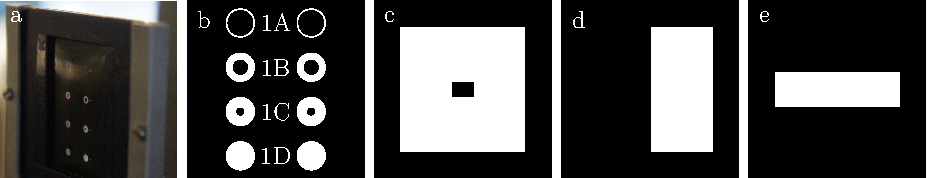
\includegraphics{images/filter/abb.pdf}
	\caption[Verwendete Filter]{
		Foto des Filterdias mit den Filtern 1A-D (a) so wie eine schematische Darstellung dieser Filter (b), sowie des Filters 2 (c), dies Halbebenfilters (d) und des Schlitzfilters (e).
	}
	\label{fig:filter}
\end{figure}


\subsection{Beugungsbild und Manipulation des Fourierhauses}

Das Fourierhaus ist ein Haus, welches aus Gittern mit gleichen Gitterkonstanten und unterschiedlichen Ausrichtungen dieser Gitter besteht (Abb.~\ref{fig:fourierhaus_mit_filtern}~a2). Die verschiedenen Gitter entsprechen verschiedenen Bauelementen im Haus. Die Wand besteht aus einem vertikalen Gitter, das Dach aus einem horizontalen Gitter und die Tür und der Schornstein werden aus diagonalen Gittern in entgegen gesetzten Richtungen erstellt. Die Fouriertransformation dieses Fourierhauses ergibt das in Abbildung~\ref{fig:fourierhaus_mit_filtern}~a1 dargestellte Beugungsbild.

\begin{figure}[h]
	\centering
	%\includegraphicsRS[width=0.75\textwidth]{images/Regina/abb21.jpg}
	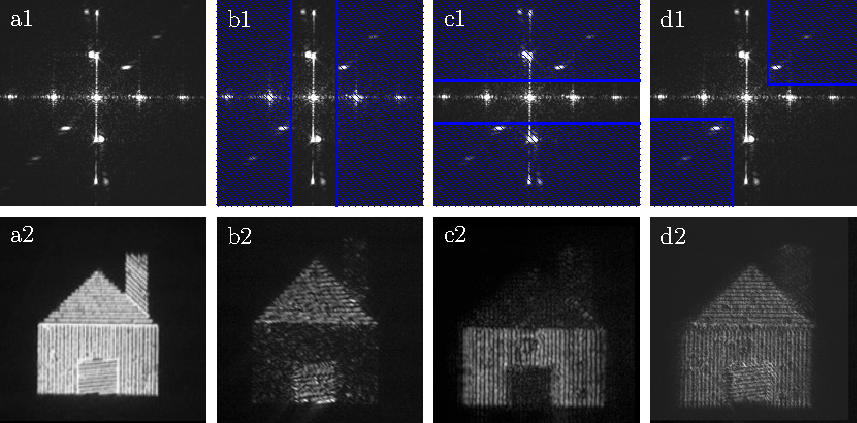
\includegraphics[scale=1]{images/Regina/abb21.pdf}
	
	\caption[Fourierhaus mit verschiedenen Filtern]{
		Durch zwei Schneiden (blau schraffiert) werden verschiedene Teile der Fourierspektren in der Fourierebene herausgefiltert (oben), welches in der Abbildungsebene zum Verschwinden einzelner Teile führt (unten).
	}
	\label{fig:fourierhaus_mit_filtern}
\end{figure}

Anschließend wurde das Fourierhaus durch Filter manipuliert. Durch die Verwendung eines Schlitzfilters (s. Abb.~\ref{fig:filter}~e), welcher bestimmte Frequenzbereiche durch Abdecken der entsprechenden Frequenzspektren herausfiltert, konnten verschiedene Bauelemente des Hauses jeweils herausgefiltert werden. Mit diesem Filter wurde das Beugungsbild in der Fourierebene so abgedeckt, dass lediglich das vertikale Fourierspektrum des Dachs und das diagonale Fourierspektrum der Tür offen blieben (Abb.~\ref{fig:fourierhaus_mit_filtern}~b1). Somit waren in der Abbildungsebene nur die horizontalen Linien des Dachs und näherungsweise horizontalen Linien der Tür sichtbar (Abb.~\ref{fig:fourierhaus_mit_filtern}~b2). Analog wurde mit Hilfe des Filters anschließend nur das horizontale Fourierspektrum geöffnet und somit nur vertikale Linien (Wand) in der Abbildungsebene sichtbar gemacht (Abb.~\ref{fig:fourierhaus_mit_filtern}~c1, c2). Als Letztes wurde durch Blockieren (mit Papierstücken) des diagonalen Fourierspektrums lediglich der Schonstein ausgeblendet (Abb.~\ref{fig:fourierhaus_mit_filtern}~d1, d2).

\subsubsection*{Auswertung}
Die vier verschiedenen Orientierungen der Gitter sind in der Fourierebene durch die vier verschiedenen Orientierungen der Punktreihen aus Intensitätsmaxima und -minima dargestellt. Auch hier stellen diese die Summe der Beugungsbilder der einzelnen Gittern dar. Da die Gitterkonstante des Fourierhauses im Vergleich zu den in Abbildung~\ref{fig:gitter_und_spektrum} und \ref{fig:kreuzgitter_und_spektrum} gezeigten Gittern sehr viel kleiner ist, sind die Abstände zwischen den Maxima im Fourierspektrum deutlich größer und die Intensität im Zentrum erhöht.


\subsection{Optische Filterung durch Hochpass-, Tiefpass- und Breitbandfilter}

%In diesem Abschnitt wird die Manipulation von Abbildungen verschiedener Objekte in der Abbildungsebene durch das Einsetzen verschiedener Filter in die Fourierebene untersucht.
In diesem Abschnitt soll der Nutzen der FT für die Bildverarbeitung illustriert werden. Dazu wurde zunächst ein Dia mit einem Fettabdruck eines Fingers präperiert. Von dieser wurde die Abbildung ohne Filter aufgenommen. Hierbei war in der Abbildungsebene relativ wenig zu erkennen (s. Abb.~\ref{fig:example20_Hochpass}~a). Anschließend wurde die Abbildung mit einem in der Fourierebene befindlichen Hochpass- und einem Halbebenenfilter (s. Abb.~\ref{fig:filter}~c, d) aufgenommen. Zudem wurde mit der Kamera 2 das Fourierspektrum des Fingerabdrucks photographiert. Zu beobachten war hier, dass die Konturen des Fingerabdrucks in der Abbildung mit Hilfe der Filter deutlich besser erkennbar gemacht werden konnten (vgl. Abbildung \ref{fig:example20_Hochpass}~b, c).

\begin{figure}[h]
	\centering
	%\includegraphicsRS[width=0.6\linewidth]{images/example20_Hochpass.png}\\
	%\includegraphicsRS[width=0.6\linewidth]{images/example21_Halbebenenfilter.png}
	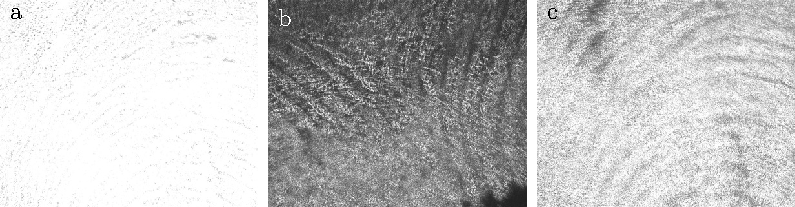
\includegraphics{images/ergebniss_Fingerab/abb.pdf}
	%TODO: Nur eines dieser Bilder!
	\caption{
		Der Fettabdruck eines Fingers in der Abbildungsebene ohne Filter (a) und mit Hochpassfiltern (b, c).
	}
	\label{fig:example20_Hochpass}
\end{figure}

Als nächstes Beispiel wurden mit der Zahl vier und dem Buchstaben D in der Objektebene Bandfilter A, B, C  sowie ein Tiefpassfilter D (s. Abb.~\ref{fig:filter}~b) in die Fourierebene eingesetzt. Bei den Bandfiltern werden die Flächen unterdrückt und Ränder als Doppellinien dargestellt. Beim Breitbandfilter 1C konnte dieser Effekt am besten beobachtet werden (Abb.~\ref{fig:vier_mit_breitband}~b). Bei den Bandfiltern 1B und 1A ist die Zahl vier kaum noch zu erkennen (Abb. \ref{fig:vier_mit_breitband}c, d). Analoge Beobachtungen waren bei dem Buchstaben D zu erkennen (s. Abb.~\ref{fig:example10_D_filter}).

\begin{figure}[h]
	\centering
	%\includegraphicsRS[width=0.4\textwidth]{images/Regina/abb22.jpg}
	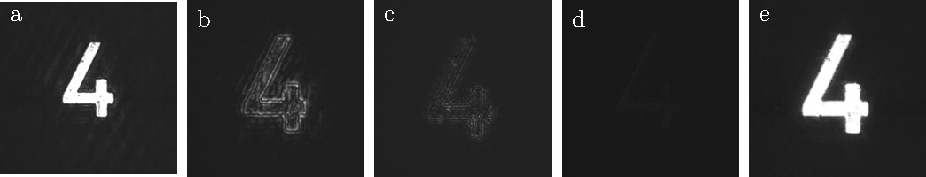
\includegraphics{images/Regina/abb22.pdf}
	\caption[Zahl 4 mit Breitbandfiltern]{
		Die Zahl vier in  der Abbildungsebene ohne Filter (a) und mit den Bandpassfiltern C (b), B (c), A (d) sowie dem Hochpassfilter D (e) manipulierte Bilder der Zahl vier.
	}
	\label{fig:vier_mit_breitband}
\end{figure}

\begin{figure}[h]
	\centering
	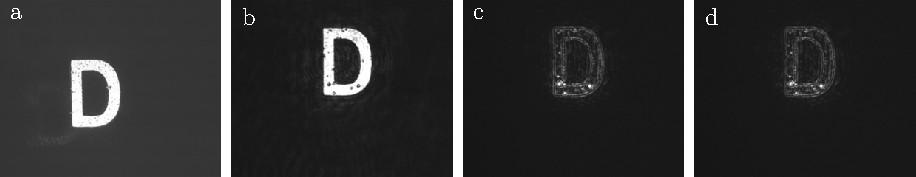
\includegraphics{images/ergebniss_D/abb.pdf}
	\caption{
		Der Buchstabe D des Objekts 4 in der Abbildungsebene ohne Filter (a), mit dem Filter 1D (b), 1C (c), 1B (d).
	}
	\label{fig:example10_D_filter}
\end{figure}


\subsubsection*{Auswertung}

Die Bandfilter lassen einen bestimmten Frequenzbereich durch. Dadurch werden sowohl sehr tiefe Frequenzen (Flächen) als auch sehr hohe Frequenzen (Kanten) unterdrückt. Die Frequenzbereiche dazwischen werden jedoch hindurch gelassen, daher prägen sich innerhalb und außerhalb der Kanten Konturlinien aus. Dies ist sowohl für die Zahl 4 als auch den Buchstaben D mit dem Filter C sehr schön zu erkennen. Die Filter A und B lassen nur sehr wenig Licht durch. Da die automatische Kontrastfunktion der Kamerasoftware nicht genutzt wurde, ist auf diesen Bildern nur mit Mühe dieser Effekt erkennen.

Durch die Verwendung eines Tiefpassfilters wurden nur die niedrigen Frequenzen durchgelassen und die hohen Frequenzen herausgefiltert. Dies bewirkt ein Verschwinden der hohen Frequenzen und so ein Verschwimmen der Kanten. Dieser weichzeichnende Effekt ist bei der Zahl 4 sehr schön zu erkennen.

Im Gegensatz dazu wurde für das Bild des Fingerabdrucks und des Buchstabens D ein Hochpassfilter eingesetzt, welcher die niedrigen Frequenzen herausfiltert, was zu einer Hervorhebung der Kanten führte.

In der Bildverarbeitung werden die Tiefpass- (Weichzeichner) und Hochpassfilter (Kantenerkennung) häufig verwendet.


\subsection{Schlierenverfahren}
Als Letztes wurde ein Teelicht auf die Position des Objektträgers gestellt und ein Halbebenenfilter in der Fourierebene installiert. Mit Kamera 1 wurden mehrere Abbildungen aufgenommen, um die Strömungsbewegungen oberhalb der Flamme beobachten zu können. Zum Vergleich wurde zudem eine Aufnahme mit Halbebenenfilter, ohne gemacht (s. Abb.~\ref{fig:Halbebenenfilter_mit_und_ohne_Teelicht}). Vergleicht man diese Abbildungen sind deutliche Verzerrungen des Lichts aufgrund der Luftströmungen über der Flamme des Teelichts zu erkennen. 

\begin{figure}[h]
	\centering
	%\includegraphicsRS[width=0.7\linewidth]{images/example22_Halbebenenfilter_mit_und_ohne_Teelicht.png}
	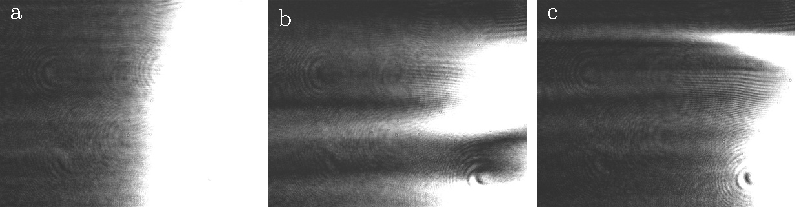
\includegraphics{images/ergebniss_Teelicht/abb.pdf}
	\caption[Schlieren]{
		Aufnahme ohne Objekt in der Abbildungsebene mit Halbebenenfilter ohne Teelicht (a) und mit Teelicht (b, c).
	}
	\label{fig:Halbebenenfilter_mit_und_ohne_Teelicht}
\end{figure}


\subsubsection*{Auswertung}
Mit Hilfe eines Halbebenenfilters wurden die durch eine brennende Kerze erzeugten Schlieren dargestellt (Abb.~\ref{fig:Halbebenenfilter_mit_und_ohne_Teelicht}). Als Schlieren werden Bereiche bezeichnet, welche sich von ihrer Umgebung in der Dichte  bzw. im Brechungsindex unterscheiden, welche in unserem Versuch die durch  die Kerze erzeugten Luftströmungen darstellten. Bei diesem Versuchsaufbau  wurde das Prinzip genutzt, dass parallele Strahlenbündel beim  Durchgang durch ein inhomogenes Dichtefeld unterschiedlich stark abgelenkt werden.   Durch den eingesetzten Halbebenenfilter, wurden die Anteile des gebrochenen  Lichts ausgeblendet, sodass richtungsabhängige Brechzahl- bzw. Dichtegradienten auf dem Projektionsschirm sichtbar wurden. Dabei ist die Intensitätsverteilung im Bild proportional zum Quadrat der Phasenverschiebung durch das Objekt. Somit ermöglicht es dieses Verfahren, eine Phasenverschiebung sichtbar zu machen.